% answers.tex —— 2011 年·浙江卷·文科 · 参考答案与详细解析片段
% 由 tools/generate_projects.py 依来源总账自 2011/2011_数学真题_浙江文_试题.md + 2011/2011_数学真题_浙江文_解析正文.md + 2011/2011_数学真题_浙江文_答案要点.md 生成，勿手改（改源 MD 后重跑）

\begin{answer}
\gksolhead{1}{}

\textbf{题目}：

若 $P=\{x\mid x<1\}$，$Q=\{x\mid x>-1\}$，则\mbox{（　　）}

（A）$P\subseteq Q$

（B）$Q\subseteq P$

（C）$\complement_{\mathbf R}P\subseteq Q$

（D）$Q\subseteq\complement_{\mathbf R}P$

\Needspace{4\baselineskip}
\textbf{解析}
$P=(-\infty,1)$，$Q=(-1,+\infty)$，$\complement_{\mathbf R}P=[1,+\infty)\subset Q$。选 C。

\gkanswer{答案：C。}

\end{answer}
\begin{answer}
\gksolhead{2}{}

\textbf{题目}：

若复数 $z=1+\mathrm i$，$\mathrm i$ 为虚数单位，则 $(1+z)\cdot\bar z=$\mbox{（　　）}

（A）$1+3\mathrm i$

（B）$3+3\mathrm i$

（C）$3-\mathrm i$

（D）$3$

\Needspace{4\baselineskip}
\textbf{解析}
$(1+z)\bar z=(2+\mathrm i)(1-\mathrm i)=3-\mathrm i$。选 C。

\gkanswer{答案：C。}

\end{answer}
\begin{answer}
\gksolhead{3}{}

\textbf{题目}：

若实数 $x$，$y$ 满足不等式组 $\begin{cases}x+2y-5\geqslant0,\\2x+y-7\geqslant0,\\x\geqslant0,\ y\geqslant0,\end{cases}$ 则 $3x+4y$ 的最小值是\mbox{（　　）}

（A）$13$

（B）$15$

（C）$20$

（D）$28$

\Needspace{4\baselineskip}
\textbf{解析}
可行域顶点为 $(0,5)$，$(0,7)$，$(3,1)$，$(5,0)$，$(7,0)$。$3x+4y$ 在这些点的值依次为 $20,28,13,15,21$，最小值为 $13$（在 $(3,1)$）。选 A。

\gkanswer{答案：A。}

\end{answer}
\begin{answer}
\gksolhead{4}{}

\textbf{题目}：

若直线 $l$ 不平行于平面 $\alpha$，且 $l\not\subset\alpha$，则\mbox{（　　）}

（A）$\alpha$ 内的所有直线与 $l$ 异面

（B）$\alpha$ 内不存在与 $l$ 平行的直线

（C）$\alpha$ 内存在唯一的直线与 $l$ 平行

（D）$\alpha$ 内的直线与 $l$ 都相交

\Needspace{4\baselineskip}
\textbf{解析}
$l$ 不平行于 $\alpha$ 且不在 $\alpha$ 内，故 $l$ 与 $\alpha$ 相交。若 $\alpha$ 内有直线与 $l$ 平行，则该直线方向与 $\alpha$ 平行，从而 $l$ 平行于 $\alpha$，矛盾；故 $\alpha$ 内不存在与 $l$ 平行的直线。选 B。

\gkanswer{答案：B。}

\end{answer}
\begin{answer}
\gksolhead{5}{}

\textbf{题目}：

在 $\triangle ABC$ 中，角 $A$，$B$，$C$ 所对的边分别为 $a$，$b$，$c$。若 $a\cos A=b\sin B$，则 $\sin A\cos A+\cos^2B=$\mbox{（　　）}

（A）$-\dfrac12$

（B）$\dfrac12$

（C）$-1$

（D）$1$

\Needspace{4\baselineskip}
\textbf{解析}
\Needspace{5\baselineskip}
由正弦定理 $a=2R\sin A$，$b=2R\sin B$，条件化为 $\sin^2A=\sin^2B$。于是
\nopagebreak[4]
\[\sin A\cos A+\cos^2B=\sin^2B+\cos^2B=1.\]
选 D。

\gkanswer{答案：D。}

\end{answer}
\begin{answer}
\gksolhead{6}{}

\textbf{题目}：

若 $a$，$b$ 为实数，则“$0<ab<1$”是“$b<\dfrac1a$”的\mbox{（　　）}

（A）充分而不必要条件

（B）必要而不充分条件

（C）充分必要条件

（D）既不充分也不必要条件

\Needspace{4\baselineskip}
\textbf{解析}
取 $a=b=-\dfrac12$，则 $0<ab<1$ 成立，但 $b=-\dfrac12<\dfrac1a=-2$ 不成立，故不充分。取 $a=1,b=2$，则 $b<\dfrac1a$ 不成立；取 $a=-1,b=0$，则 $b< -1$ 不成立。再取 $a=-1,b=-2$：$b<\dfrac1a$（$-2<-1$）成立，但 $ab=2>1$，故不必要。选 D。

\gkanswer{答案：D。}

\end{answer}
\begin{answer}
\gksolhead{7}{}

\textbf{题目}：

若某几何体的三视图如图所示，则这个几何体的直观图可以是\mbox{（　　）}

（A）图 A

（B）图 B

（C）图 C

（D）图 D
\nopagebreak[4]
\begin{center}% 2011 年浙江卷文科第 7 题：三视图与四个直观图选项。
% 来源 PDF：普通高考/2011/2011浙江文.pdf，SHA-256 36931500dfd850579d93f0a685f0ccea25065c84c09db5157c451093d53b56f0。
% 原页：第 1 页第 1 栏，书页码 711。示意图。
\begin{tikzpicture}[>=stealth, semithick, font=\small, scale=0.85]
  \draw[thick] (0,0) rectangle (1.6,1.6);
  \draw[thick] (0,0.8)--(1.6,0.8);
  \node[below] at (0.8,-0.1) {正视图};
  \draw[thick] (2.4,0)--(2.4,1.6)--(3.3,1.6)--(3.8,0.9)--(3.8,0)--cycle;
  \node[below] at (3.1,-0.1) {侧视图};
  \draw[thick] (0.2,-2.4) rectangle (1.8,-0.8);
  \draw[thick] (0.2,-1.6)--(1.8,-1.6);
  \node[below] at (1.0,-2.5) {俯视图};
  % 选项
  \begin{scope}[xshift=4.2cm, yshift=-2.4cm, scale=0.5]
    \draw[thick] (0,0)--(2,0)--(2,1.2)--(0,1.2)--cycle;
    \draw[thick] (0,1.2)--(0.5,2.4)--(2.6,1.5)--(2,1.2);
    \draw[thick] (2,0)--(2.6,0.3)--(2.6,1.5);
    \node[below] at (1,-0.4) {(A)};
  \end{scope}
  \begin{scope}[xshift=7.4cm, yshift=-2.4cm, scale=0.5]
    \draw[thick] (0,0)--(2,0)--(2,1.2)--(0,1.2)--cycle;
    \draw[thick] (0,1.2)--(2,2.0)--(2.6,1.5)--(2,1.2);
    \draw[thick] (2,0)--(2.6,0.3)--(2.6,1.5);
    \node[below] at (1,-0.4) {(B)};
  \end{scope}
  \begin{scope}[xshift=10.6cm, yshift=-2.4cm, scale=0.5]
    \draw[thick] (0,0)--(2,0)--(2,1.2)--(0,1.2)--cycle;
    \draw[thick] (0.2,1.2)--(1.0,2.4)--(1.8,1.2);
    \draw[thick] (2,0)--(2.6,0.3)--(2.6,1.5)--(2,1.2);
    \node[below] at (1,-0.4) {(C)};
  \end{scope}
  \begin{scope}[xshift=13.8cm, yshift=-2.4cm, scale=0.5]
    \draw[thick] (0,0)--(2,0)--(2,1.2)--(0,1.2)--cycle;
    \draw[thick] (0,1.2)--(2,1.2)--(2,2.0)--(0,2.0)--cycle;
    \draw[thick] (2,0)--(2.6,0.3)--(2.6,2.3)--(2,2.0);
    \draw[thick] (0,2.0)--(0.6,2.3)--(2.6,2.3);
    \node[below] at (1,-0.4) {(D)};
  \end{scope}
\end{tikzpicture}
\end{center}
\nopagebreak[4]
\Needspace{4\baselineskip}
\textbf{解析}
正视图为上下两个矩形，说明前方有一水平棱；侧视图上缘为左上高、右下低的斜线；俯视图为前后两个矩形。四个直观图中只有（B）的顶部为前低后高的斜面、正面被一条水平棱分为上下两部分。选 B。

\gkanswer{答案：B。}

\end{answer}
\begin{answer}
\gksolhead{8}{}

\textbf{题目}：

从装有 $3$ 个红球、$2$ 个白球的袋中任取 $3$ 个球，则所取的 $3$ 个球中至少有 $1$ 个白球的概率是\mbox{（　　）}

（A）$\dfrac1{10}$

（B）$\dfrac3{10}$

（C）$\dfrac35$

（D）$\dfrac9{10}$

\Needspace{4\baselineskip}
\textbf{解析}
\Needspace{5\baselineskip}
任取 $3$ 球共 $\mathrm C_5^3=10$ 种。全是红球只有 $1$ 种，故至少一个白球概率
\nopagebreak[4]
\[1-\frac1{10}=\frac9{10}.\]
选 D。

\gkanswer{答案：D。}

\end{answer}
\begin{answer}
\gksolhead{9}{}

\textbf{题目}：

已知椭圆 $C_1:\dfrac{x^2}{a^2}+\dfrac{y^2}{b^2}=1$（$a>b>0$）与双曲线 $C_2:x^2-\dfrac{y^2}4=1$ 有公共的焦点，$C_2$ 的一条渐近线与以 $C_1$ 的长轴为直径的圆相交于 $A$，$B$ 两点。若 $C_1$ 恰好将线段 $AB$ 三等分，则\mbox{（　　）}

（A）$a^2=\dfrac{13}2$

（B）$a^2=13$

（C）$b^2=\dfrac12$

（D）$b^2=2$

\Needspace{4\baselineskip}
\textbf{解析}
双曲线 $x^2-\dfrac{y^2}4=1$ 的 $c^2=5$，故椭圆 $a^2-b^2=5$。渐近线 $y=2x$ 与圆 $x^2+y^2=a^2$ 交于直径 $AB$，长 $2a$。
\Needspace{5\baselineskip}
椭圆与该直线交点满足
\nopagebreak[4]
\[\frac{x^2}{a^2}+\frac{4x^2}{b^2}=1\Longrightarrow x^2=\frac{a^2b^2}{b^2+4a^2}.\]
\Needspace{5\baselineskip}
椭圆将 $AB$ 三等分，即截得弦长为 $\dfrac{2a}3$；弦端点到圆心距离为 $\dfrac a3$，而直线上点 $(x,2x)$ 到圆心距离为 $\sqrt5|x|$，故 $x^2=\dfrac{a^2}{45}$。于是
\nopagebreak[4]
\[\frac{b^2}{b^2+4a^2}=\frac1{45}\Longrightarrow a^2=11b^2.\]
结合 $a^2-b^2=5$ 得 $b^2=\dfrac12$。选 C。

\gkanswer{答案：C。}

\end{answer}
\begin{answer}
\gksolhead{10}{}

\textbf{题目}：

设函数 $f(x)=ax^2+bx+c$（$a$，$b$，$c\in\mathbf R$）。若 $x=-1$ 为函数 $y=f(x)\mathrm e^x$ 的一个极值点，则下列图象不可能为 $y=f(x)$ 图象的是\mbox{（　　）}

（A）图 A

（B）图 B

（C）图 C

（D）图 D
\nopagebreak[4]
\begin{center}% 2011 年浙江卷文科第 10 题：四个 y=f(x) 图象选项。
% 来源 PDF：普通高考/2011/2011浙江文.pdf，SHA-256 36931500dfd850579d93f0a685f0ccea25065c84c09db5157c451093d53b56f0。
% 原页：第 1 页第 2 栏，书页码 711。示意图；x=-1 用虚线标出。
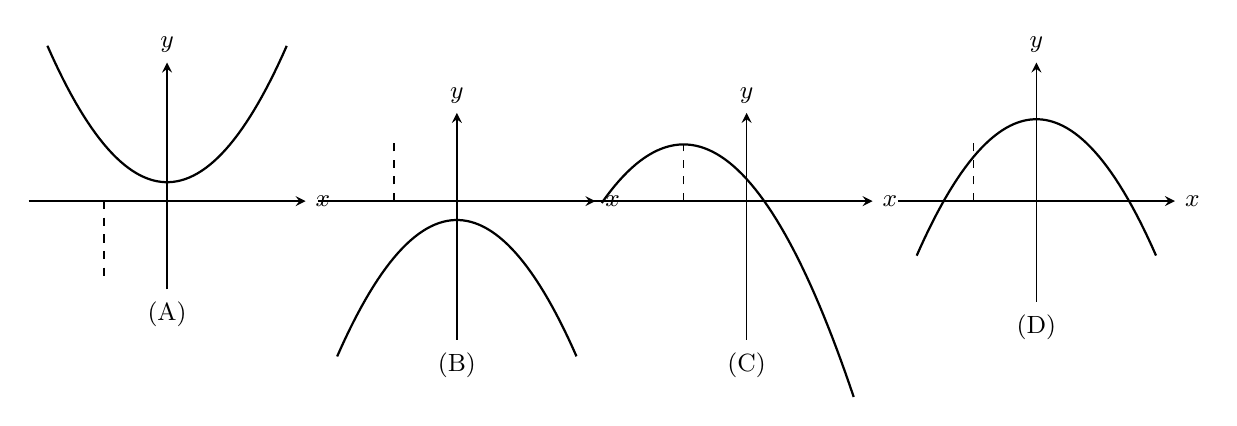
\begin{tikzpicture}[>=stealth, semithick, font=\small, scale=0.8]
  % (A) 开口向上，截距正
  \begin{scope}
    \draw[->] (-2.2,0)--(2.2,0) node[right] {$x$};
    \draw[->] (0,-1.4)--(0,2.2) node[above] {$y$};
    \draw[dashed] (-1,0)--(-1,-1.2);
    \draw[thick, domain=-1.9:1.9, samples=60] plot (\x,{0.6*\x*\x+0.3});
    \node at (0,-1.8) {(A)};
  \end{scope}
  % (B) 开口向下，截距负
  \begin{scope}[xshift=4.6cm]
    \draw[->] (-2.2,0)--(2.2,0) node[right] {$x$};
    \draw[->] (0,-2.2)--(0,1.4) node[above] {$y$};
    \draw[dashed] (-1,0)--(-1,1.0);
    \draw[thick, domain=-1.9:1.9, samples=60] plot (\x,{-0.6*\x*\x-0.3});
    \node at (0,-2.6) {(B)};
  \end{scope}
  % (C) 开口向下，顶点在 x=-1 附近，截距负
  \begin{scope}[xshift=9.2cm]
    \draw[->] (-2.6,0)--(2.0,0) node[right] {$x$};
    \draw[->] (0,-2.2)--(0,1.4) node[above] {$y$};
    \draw[dashed] (-1,0)--(-1,0.9);
    \draw[thick, domain=-2.3:1.7, samples=60] plot (\x,{-0.55*(\x+1)*(\x+1)+0.9});
    \node at (0,-2.6) {(C)};
  \end{scope}
  % (D) 开口向下，但截距为正（不可能）
  \begin{scope}[xshift=13.8cm]
    \draw[->] (-2.2,0)--(2.2,0) node[right] {$x$};
    \draw[->] (0,-1.6)--(0,2.2) node[above] {$y$};
    \draw[dashed] (-1,0)--(-1,1.0);
    \draw[thick, domain=-1.9:1.9, samples=60] plot (\x,{-0.6*\x*\x+1.3});
    \node at (0,-2.0) {(D)};
  \end{scope}
\end{tikzpicture}
\end{center}
\nopagebreak[4]
\Needspace{4\baselineskip}
\textbf{解析}
\Needspace{5\baselineskip}
$g(x)=f(x)\mathrm e^x$，$g'(-1)=\mathrm e^{-1}[f(-1)+f'(-1)]=0$：
\nopagebreak[4]
\[(a-b+c)+(-2a+b)=0\Longrightarrow c=a.\]
故 $f(0)=c=a$：抛物线开口向上（$a>0$）时 $y$ 截距必为正，开口向下（$a<0$）时截距必为负。（D）中抛物线开口向下而 $y$ 截距为正，不可能。选 D。

\gkanswer{答案：D。}

\end{answer}
\begin{answer}
\gksolhead{11}{}

\textbf{题目}：

设函数 $f(x)=\dfrac4{1-x}$。若 $f(a)=2$，则实数 $a=$ $\underline{\qquad}$。

\Needspace{4\baselineskip}
\textbf{解析}
$\dfrac4{1-a}=2\Longrightarrow1-a=2\Longrightarrow a=-1$。

\gkanswer{答案：$-1$。}

\end{answer}
\begin{answer}
\gksolhead{12}{}

\textbf{题目}：

若直线 $x-2y+5=0$ 与直线 $2x+my-6=0$ 互相垂直，则实数 $m=$ $\underline{\qquad}$。

\Needspace{4\baselineskip}
\textbf{解析}
两直线垂直：$1\cdot2+(-2)m=0$，故 $m=1$。

\gkanswer{答案：$1$。}

\end{answer}
\begin{answer}
\gksolhead{13}{}

\textbf{题目}：

某小学为了解学生数学课程的学习情况，在 $3000$ 名学生中随机抽取 $200$ 名，并统计这 $200$ 名学生的某次数学考试成绩，得到了样本的频率分布直方图（如图）。根据频率分布直方图，$3000$ 名学生在该次数学考试中成绩小于 $60$ 分的学生数是 $\underline{\qquad}$。
\nopagebreak[4]
\begin{center}% 2011 年浙江卷文科第 13 题：样本频率分布直方图。
% 来源 PDF：普通高考/2011/2011浙江文.pdf，SHA-256 36931500dfd850579d93f0a685f0ccea25065c84c09db5157c451093d53b56f0。
% 原页：第 1 页第 2 栏下部，书页码 711。组距 10；<60 分组高为 0.002,0.006,0.012。
\begin{tikzpicture}[>=stealth, semithick, font=\small, x=0.9cm, y=22cm]
  \draw[->] (0,0)--(10,0) node[right] {成绩/分};
  \draw[->] (0,0)--(0,0.032) node[above] {$\dfrac{\text{频率}}{\text{组距}}$};
  \foreach \x/\h in {3/0.002,4/0.006,5/0.012,6/0.024,7/0.028}{
    \draw (\x-0.5,0) rectangle (\x+0.5,\h);
  }
  \foreach \x in {3,4,5,6,7} \node[below] at (\x,0) {$\x0$};
  \foreach \y in {0.002,0.006,0.012,0.024,0.028} \node[left] at (0,\y) {\y};
  \node[below left] at (0,0) {$O$};
\end{tikzpicture}
\end{center}
\nopagebreak[4]
\Needspace{4\baselineskip}
\textbf{解析}
\Needspace{5\baselineskip}
$<60$ 分的三个组的频率为
\nopagebreak[4]
\[10(0.002+0.006+0.012)=0.20,\]
故 $3000\times0.20=600$ 人。

\gkanswer{答案：$600$。}

\end{answer}
\begin{answer}
\gksolhead{14}{}

\textbf{题目}：

某程序框图如图所示，则该程序运行后输出的 $k$ 的值是 $\underline{\qquad}$。
\nopagebreak[4]
\begin{center}% 2011 年浙江卷理科第 12 题：程序框图。
% 来源 PDF：普通高考/2011/2011浙江理.pdf，SHA-256 0239778f574bc3ce6d7aca5024aa6333f80d131abaf699f79c46472394f8cd65。
% 原页：第 1 页第 2 栏中部，书页码 709。
\begin{tikzpicture}[>=stealth, semithick, font=\small]
  \node[draw, rounded corners=0.12cm, minimum width=1.2cm, minimum height=0.5cm] (start) at (0,0) {开始};
  \node[draw, minimum width=1.4cm, minimum height=0.5cm] (k2) at (0,-1.1) {$k=2$};
  \node[draw, minimum width=1.8cm, minimum height=0.5cm] (inc) at (0,-2.2) {$k=k+1$};
  \node[draw, minimum width=1.8cm, minimum height=0.5cm] (a) at (0,-3.3) {$a=4^k$};
  \node[draw, minimum width=1.8cm, minimum height=0.5cm] (b) at (0,-4.4) {$b=k^4$};
  \node[draw, diamond, aspect=1.7, minimum width=1.6cm, minimum height=0.9cm] (test) at (0,-5.8) {$a>b$};
  \node[draw, trapezium, trapezium left angle=72, trapezium right angle=108,
        minimum width=1.6cm, minimum height=0.55cm] (out) at (0,-7.2) {输出 $k$};
  \node[draw, rounded corners=0.12cm, minimum width=1.2cm, minimum height=0.5cm] (stop) at (0,-8.4) {结束};
  \draw[->] (start.south)--(k2.north);
  \draw[->] (k2.south)--(inc.north);
  \draw[->] (inc.south)--(a.north);
  \draw[->] (a.south)--(b.north);
  \draw[->] (b.south)--(test.north);
  \draw[->] (test.south)--(out.north) node[midway, right] {是};
  \draw[->] (out.south)--(stop.north);
  \draw[->] (test.east) -- ++(1.4,0) |- (inc.east) node[pos=0.25, right] {否};
\end{tikzpicture}
\end{center}
\nopagebreak[4]
\Needspace{4\baselineskip}
\textbf{解析}
同理科第 12 题：$k=3$ 时 $64<81$，$k=4$ 时 $256=256$，$k=5$ 时 $1024>625$，输出 $5$。

\gkanswer{答案：$5$。}

\end{answer}
\begin{answer}
\gksolhead{15}{}

\textbf{题目}：

若平面向量 $\boldsymbol\alpha$、$\boldsymbol\beta$ 满足 $|\boldsymbol\alpha|=1$，$|\boldsymbol\beta|\leqslant1$，且以向量 $\boldsymbol\alpha$、$\boldsymbol\beta$ 为邻边的平行四边形的面积为 $\dfrac12$，则 $\boldsymbol\alpha$ 和 $\boldsymbol\beta$ 的夹角 $\theta$ 的取值范围是 $\underline{\qquad}$。

\Needspace{4\baselineskip}
\textbf{解析}
\Needspace{5\baselineskip}
$|\boldsymbol\beta|\sin\theta=\dfrac12$，故 $\sin\theta=\dfrac1{2|\boldsymbol\beta|}\geqslant\dfrac12$，故
\nopagebreak[4]
\[\theta\in\left[\frac\pi6,\frac{5\pi}6\right].\]

\gkanswer{答案：$\left[\dfrac\pi6,\dfrac{5\pi}6\right]$。}

\end{answer}
\begin{answer}
\gksolhead{16}{}

\textbf{题目}：

若实数 $x$，$y$ 满足 $x^2+y^2+xy=1$，则 $x+y$ 的最大值是 $\underline{\qquad}$。

\Needspace{4\baselineskip}
\textbf{解析}
\Needspace{5\baselineskip}
令 $t=x+y$，则 $xy=t^2-1$。实数 $x,y$ 要求
\nopagebreak[4]
\[t^2\geqslant4xy=4(t^2-1)\Longrightarrow3t^2\leqslant4\Longrightarrow t\leqslant\frac{2\sqrt3}3.\]

\gkanswer{答案：$\dfrac{2\sqrt3}3$。}

\end{answer}
\begin{answer}
\gksolhead{17}{}

\textbf{题目}：

若数列 $\left\{n(n+4)\left(\dfrac23\right)^n\right\}$ 中的最大项是第 $k$ 项，则 $k=$ $\underline{\qquad}$。

\Needspace{4\baselineskip}
\textbf{解析}
\Needspace{5\baselineskip}
设 $a_n=n(n+4)\left(\dfrac23\right)^n$，则
\nopagebreak[4]
\[\frac{a_{n+1}}{a_n}=\frac{2(n+1)(n+5)}{3n(n+4)}.\]
由 $\dfrac{2(n+1)(n+5)}{3n(n+4)}\geqslant1$ 得 $n^2\leqslant10$，即 $n\leqslant3$；故数列在 $n\leqslant3$ 时递增、$n\geqslant4$ 时递减，最大项为第 $3$ 项。

\gkanswer{答案：$3$。}

\end{answer}
\begin{answer}
\gksolhead{18}{}

\textbf{题目}：

已知函数 $f(x)=A\sin\left(\dfrac\pi3x+\varphi\right)$，$x\in\mathbf R$，$A>0$，$0<\varphi<\dfrac\pi2$。$y=f(x)$ 的部分图象如图所示，$P$，$Q$ 分别为该图象的最高点和最低点，点 $P$ 的坐标为 $(1,A)$。

（1） 求 $f(x)$ 的最小正周期及 $\varphi$ 的值；

（2） 若点 $R$ 的坐标为 $(1,0)$，$\angle PRQ=\dfrac{2\pi}3$，求 $A$ 的值。
\nopagebreak[4]
\begin{center}% 2011 年浙江卷文科第 18 题：f(x)=A sin(πx/3+φ) 的部分图象。
% 来源 PDF：普通高考/2011/2011浙江文.pdf，SHA-256 36931500dfd850579d93f0a685f0ccea25065c84c09db5157c451093d53b56f0。
% 原页：第 1 页第 3 栏，书页码 711。P(1,A) 最高点，Q(4,-A) 最低点，R(1,0)。
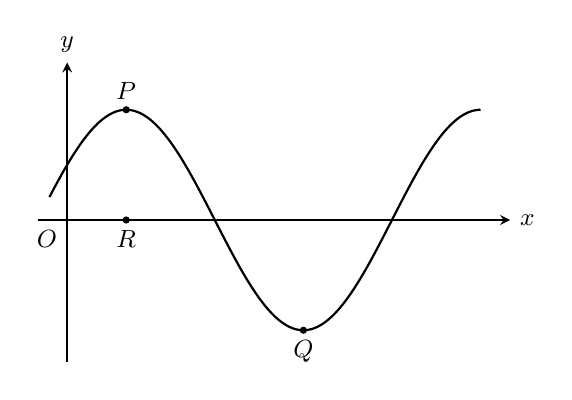
\begin{tikzpicture}[>=stealth, semithick, font=\small, x=0.75cm, y=1.0cm]
  \draw[->] (-0.5,0)--(7.5,0) node[right] {$x$};
  \draw[->] (0,-1.8)--(0,2.0) node[above] {$y$};
  \node[below left] at (0,0) {$O$};
  \draw[thick, domain=-0.3:7.0, samples=200] plot (\x,{1.4*sin(deg(pi*\x/3+pi/6))});
  \fill (1,1.4) circle (1.3pt) node[above] {$P$};
  \fill (4,-1.4) circle (1.3pt) node[below] {$Q$};
  \fill (1,0) circle (1.3pt) node[below] {$R$};
\end{tikzpicture}
\end{center}
\nopagebreak[4]
\Needspace{4\baselineskip}
\textbf{解析}
\gksubpart{(1)}
\Needspace{5\baselineskip}
$\omega=\dfrac\pi3$，故 $T=\dfrac{2\pi}{\omega}=6$。最高点 $P(1,A)$，故
\nopagebreak[4]
\[\frac\pi3\cdot1+\varphi=\frac\pi2+2k\pi\Longrightarrow\varphi=\frac\pi6.\]

\gksubpart{(2)}
\Needspace{5\baselineskip}
最低点 $Q$ 的横坐标为 $1+\dfrac T2=4$，故 $Q(4,-A)$。$R(1,0)$，
\nopagebreak[4]
\[\overrightarrow{RP}=(0,A),\qquad\overrightarrow{RQ}=(3,-A).\]
\nopagebreak[4]
\[\cos\angle PRQ=\frac{-A^2}{A\sqrt{9+A^2}}=-\frac{A}{\sqrt{9+A^2}}=\cos\frac{2\pi}3=-\frac12,\]
故 $4A^2=9+A^2$，$A^2=3$，$A=\sqrt3$。

\gkanswer{答案（1）：$T=6$，$\varphi=\dfrac\pi6$。}

\gkanswer{答案（2）：$A=\sqrt3$。}

\end{answer}
\begin{answer}
\gksolhead{19}{}

\textbf{题目}：

已知公差不为 $0$ 的等差数列 $\{a_n\}$ 的首项 $a_1$ 为 $a$（$a\in\mathbf R$），且 $\dfrac1{a_1}$，$\dfrac1{a_2}$，$\dfrac1{a_4}$ 成等比数列。

（1） 求数列 $\{a_n\}$ 的通项公式；

（2） 对 $n\in\mathbf N^*$，试比较 $\dfrac1{a_2}+\dfrac1{a_{2^2}}+\dfrac1{a_{2^3}}+\cdots+\dfrac1{a_{2^n}}$ 与 $\dfrac1{a_1}$ 的大小。

\Needspace{4\baselineskip}
\textbf{解析}
\gksubpart{(1)}
$\dfrac1{a_1},\dfrac1{a_2},\dfrac1{a_4}$ 成等比，故 $a_2^2=a_1a_4$。设公差 $d\neq0$，则 $(a+d)^2=a(a+3d)$，得 $d^2=ad$，$d=a$。故 $a_n=na$。

\gksubpart{(2)}
\Needspace{5\baselineskip}
$a_{2^k}=2^ka$，故
\nopagebreak[4]
\[\sum_{k=1}^n\frac1{a_{2^k}}=\frac1a\sum_{k=1}^n\frac1{2^k}=\frac1a\left(1-\frac1{2^n}\right)<\frac1a=\frac1{a_1}.\]

\gkanswer{答案（1）：$a_n=na$。}

\gkanswer{答案（2）：$\dfrac1{a_2}+\dfrac1{a_{2^2}}+\cdots+\dfrac1{a_{2^n}}<\dfrac1{a_1}$。}

\end{answer}
\begin{answer}
\gksolhead{20}{}

\textbf{题目}：

如图，在三棱锥 $P-ABC$ 中，$AB=AC$，$D$ 为 $BC$ 的中点，$PO\perp$ 平面 $ABC$，垂足 $O$ 落在线段 $AD$ 上。

（1） 证明：$AP\perp BC$；

（2） 已知 $BC=8$，$PO=4$，$AO=3$，$OD=2$，求二面角 $B-AP-C$ 的大小。
\nopagebreak[4]
\begin{center}% 2011 年浙江卷理科第 20 题：三棱锥 P-ABC，O 在 AD 上，PO⊥平面 ABC。
% 来源 PDF：普通高考/2011/2011浙江理.pdf，SHA-256 0239778f574bc3ce6d7aca5024aa6333f80d131abaf699f79c46472394f8cd65。
% 原页：第 2 页第 1 栏，书页码 710。示意。
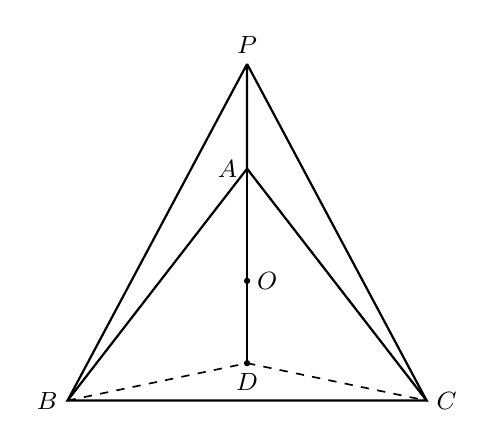
\begin{tikzpicture}[>=stealth, semithick, font=\small, scale=0.95]
  \coordinate (D) at (0,0);
  \coordinate (B) at (-2.4,-0.5);
  \coordinate (C) at (2.4,-0.5);
  \coordinate (A) at (0,2.6);
  \coordinate (O) at (0,1.1);
  \coordinate (P) at (0,4.0);
  \draw[thick] (A)--(B)--(C)--cycle;
  \draw[thick] (P)--(A) (P)--(B) (P)--(C);
  \draw[dashed] (A)--(C);
  \draw[dashed] (P)--(O);
  \draw[dashed] (B)--(D);
  \draw[dashed] (D)--(C);
  \draw (A)--(D);
  \fill (D) circle (1.2pt) node[below] {$D$};
  \fill (O) circle (1.2pt) node[right] {$O$};
  \node[left] at (A) {$A$};
  \node[left] at (B) {$B$};
  \node[right] at (C) {$C$};
  \node[above] at (P) {$P$};
\end{tikzpicture}
\end{center}
\nopagebreak[4]
\Needspace{4\baselineskip}
\textbf{解析}
\gksubpart{(1)}
$AB=AC$，$D$ 为 $BC$ 中点，故 $AD\perp BC$；又 $PO\perp$ 平面 $ABC$，故 $PO\perp BC$。于是 $BC\perp$ 平面 $PAD$，从而 $BC\perp AP$。

\gksubpart{(2)}
\Needspace{5\baselineskip}
以 $D$ 为原点，$DB$、$DA$ 分别为 $x$、$y$ 轴建立坐标系：
\nopagebreak[4]
\[D(0,0,0),\ B(4,0,0),\ C(-4,0,0),\ A(0,-5,0),\ P(0,-2,4).\]
\Needspace{5\baselineskip}
平面 $BAP$ 的法向量
\nopagebreak[4]
\[\boldsymbol n_1=\overrightarrow{AB}\times\overrightarrow{AP}=(4,5,0)\times(0,3,4)=(20,-16,12)\sim(5,-4,3),\]
\Needspace{5\baselineskip}
平面 $CAP$ 的法向量
\nopagebreak[4]
\[\boldsymbol n_2=\overrightarrow{AC}\times\overrightarrow{AP}=(-4,5,0)\times(0,3,4)=(20,16,-12)\sim(5,4,-3).\]
$\boldsymbol n_1\cdot\boldsymbol n_2=25-16-9=0$，故二面角 $B-AP-C$ 为 $90^\circ$。

\gkanswer{答案（1）：证明见解析。}

\gkanswer{答案（2）：$90^\circ$。}

\end{answer}
\begin{answer}
\gksolhead{21}{}

\textbf{题目}：

设函数 $f(x)=a^2\ln x-x^2+ax$，$a>0$。

（1） 求 $f(x)$ 的单调区间；

（2） 求所有实数 $a$，使 $\mathrm e-1\leqslant f(x)\leqslant\mathrm e^2$ 对 $x\in[1,\mathrm e]$ 恒成立。

注：$\mathrm e$ 为自然对数的底数。

\Needspace{4\baselineskip}
\textbf{解析}
\gksubpart{(1)}
\nopagebreak[4]
\[f'(x)=\frac{a^2}{x}-2x+a=\frac{-2x^2+ax+a^2}{x}=-\frac{(2x+a)(x-a)}x.\]
$a>0$，$x>0$ 时 $2x+a>0$，故 $0<x<a$ 时 $f'>0$，$x>a$ 时 $f'<0$。增区间 $(0,a)$，减区间 $(a,+\infty)$。

\gksubpart{(2)}
由（1）$f$ 在 $[1,\mathrm e]$ 上的最大值与最小值需满足 $\mathrm e-1\leqslant f\leqslant\mathrm e^2$。
若 $a\leqslant1$，$f$ 在 $[1,\mathrm e]$ 递减，最小值为 $f(\mathrm e)=a^2-\mathrm e^2+a\mathrm e<0<\mathrm e-1$，不合。
若 $1<a\leqslant\mathrm e$，最大值 $f(a)=a^2\ln a\leqslant\mathrm e^2$ 要求 $a\leqslant\mathrm e$；最小值 $\min\{f(1),f(\mathrm e)\}$。$f(1)=a-1\geqslant\mathrm e-1$ 要求 $a\geqslant\mathrm e$，故 $a=\mathrm e$。
若 $a>\mathrm e$，$f$ 在 $[1,\mathrm e]$ 递减，最大 $f(1)=a-1\leqslant\mathrm e^2$ 要求 $a\leqslant\mathrm e^2+1$；最小 $f(\mathrm e)=a^2-\mathrm e^2+a\mathrm e\geqslant\mathrm e-1$，在 $a>\mathrm e$ 时成立。
综上 $a\in[\mathrm e,\mathrm e^2+1]$。

\gkanswer{答案（1）：在 $(0,a)$ 上递增，在 $(a,+\infty)$ 上递减。}

\gkanswer{答案（2）：$[\mathrm e,\mathrm e^2+1]$。}

\end{answer}
\begin{answer}
\gksolhead{22}{}

\textbf{题目}：

如图，设 $P$ 为抛物线 $C_1:x^2=y$ 上的动点，过点 $P$ 作圆 $C_2:x^2+(y+3)^2=1$ 的两条切线，交直线 $l:y=-3$ 于 $A$，$B$ 两点。

（1） 求 $C_2$ 的圆心 $M$ 到抛物线 $C_1$ 准线的距离。

（2） 是否存在点 $P$，使线段 $AB$ 被抛物线 $C_1$ 在点 $P$ 处的切线平分？若存在，求出点 $P$ 的坐标；若不存在，请说明理由。
\nopagebreak[4]
\begin{center}% 2011 年浙江卷文科第 22 题：抛物线 x^2=y、圆 x^2+(y+3)^2=1、直线 y=-3。
% 来源 PDF：普通高考/2011/2011浙江文.pdf，SHA-256 36931500dfd850579d93f0a685f0ccea25065c84c09db5157c451093d53b56f0。
% 原页：第 2 页第 3 栏，书页码 712。示意图。
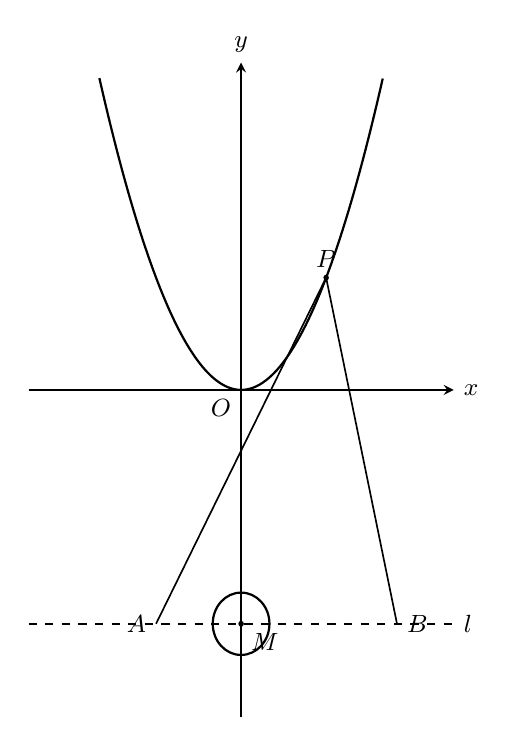
\begin{tikzpicture}[>=stealth, semithick, font=\small, scale=0.9, yscale=1.1]
  \draw[->] (-3,0)--(3,0) node[right] {$x$};
  \draw[->] (0,-4.2)--(0,4.2) node[above] {$y$};
  \draw[thick, domain=-2:2, samples=100] plot (\x,{\x*\x});
  \draw[thick] (0,-3) circle (0.4);
  \fill (0,-3) circle (1.1pt) node[below right] {$M$};
  \draw[dashed] (-3,-3)--(3,-3) node[right] {$l$};
  \coordinate (P) at (1.2,1.44);
  \fill (P) circle (1.1pt) node[above] {$P$};
  \draw (P)--(-1.2,-3) node[left] {$A$};
  \draw (P)--(2.2,-3) node[right] {$B$};
  \node[below left] at (0,0) {$O$};
\end{tikzpicture}
\end{center}
\nopagebreak[4]
\Needspace{4\baselineskip}
\textbf{解析}
\gksubpart{(1)}
\Needspace{5\baselineskip}
抛物线 $x^2=y$ 的准线为 $y=-\dfrac14$，圆心 $M(0,-3)$ 到准线距离
\nopagebreak[4]
\[-3-\left(-\frac14\right)=-\frac{11}4\text{ \text{的绝对值}}=\frac{11}4.\]

\gksubpart{(2)}
\Needspace{5\baselineskip}
设 $P(t,t^2)$，过 $P$ 的切线为 $y=2tx-t^2$，与 $y=-3$ 交于
\nopagebreak[4]
\[X\left(\frac{t^2-3}{2t},-3\right).\]
\Needspace{5\baselineskip}
设过 $P$ 的切线与 $y=-3$ 交于 $A,B$，切线斜率 $m$ 满足到圆心 $M(0,-3)$ 的距离为 $1$：
\nopagebreak[4]
\[(t^2+3-mt)^2=m^2+1,\]
\Needspace{5\baselineskip}
即
\nopagebreak[4]
\[(t^2-1)m^2-2t(t^2+3)m+(t^2+3)^2-1=0.\]
\Needspace{5\baselineskip}
交点横坐标 $x=t-\dfrac{t^2+3}{m}$，故 $AB$ 中点横坐标为
\nopagebreak[4]
\[x_0=t-\frac{t^2+3}{2}\left(\frac1{m_1}+\frac1{m_2}\right).\]
\Needspace{5\baselineskip}
由韦达定理
\nopagebreak[4]
\[\frac1{m_1}+\frac1{m_2}=\frac{2t(t^2+3)}{(t^2+2)(t^2+4)},\]
\Needspace{5\baselineskip}
故
\nopagebreak[4]
\[x_0=t\left[1-\frac{(t^2+3)^2}{(t^2+2)(t^2+4)}\right]
=-\frac{t}{(t^2+2)(t^2+4)}.\]
\Needspace{5\baselineskip}
中点落在切线上，故 $x_0=\dfrac{t^2-3}{2t}$：
\nopagebreak[4]
\[-\frac{t}{(t^2+2)(t^2+4)}=\frac{t^2-3}{2t}.\]
\Needspace{5\baselineskip}
令 $u=t^2$，化简得
\nopagebreak[4]
\[u^3+3u^2-8u-24=0\Longrightarrow(u+3)(u^2-8)=0,\]
\Needspace{5\baselineskip}
故 $u=2\sqrt2$，$t=\pm2^{3/4}$。存在，且
\nopagebreak[4]
\[P\left(\pm2^{3/4},2\sqrt2\right).\]

\gkanswer{答案（1）：$\dfrac{11}4$。}

\gkanswer{答案（2）：存在，$P\left(\pm2^{3/4},2\sqrt2\right)$。}

\end{answer}